\begin{figure*}
	\centering
    \resizebox{1.5\columnwidth}{!}{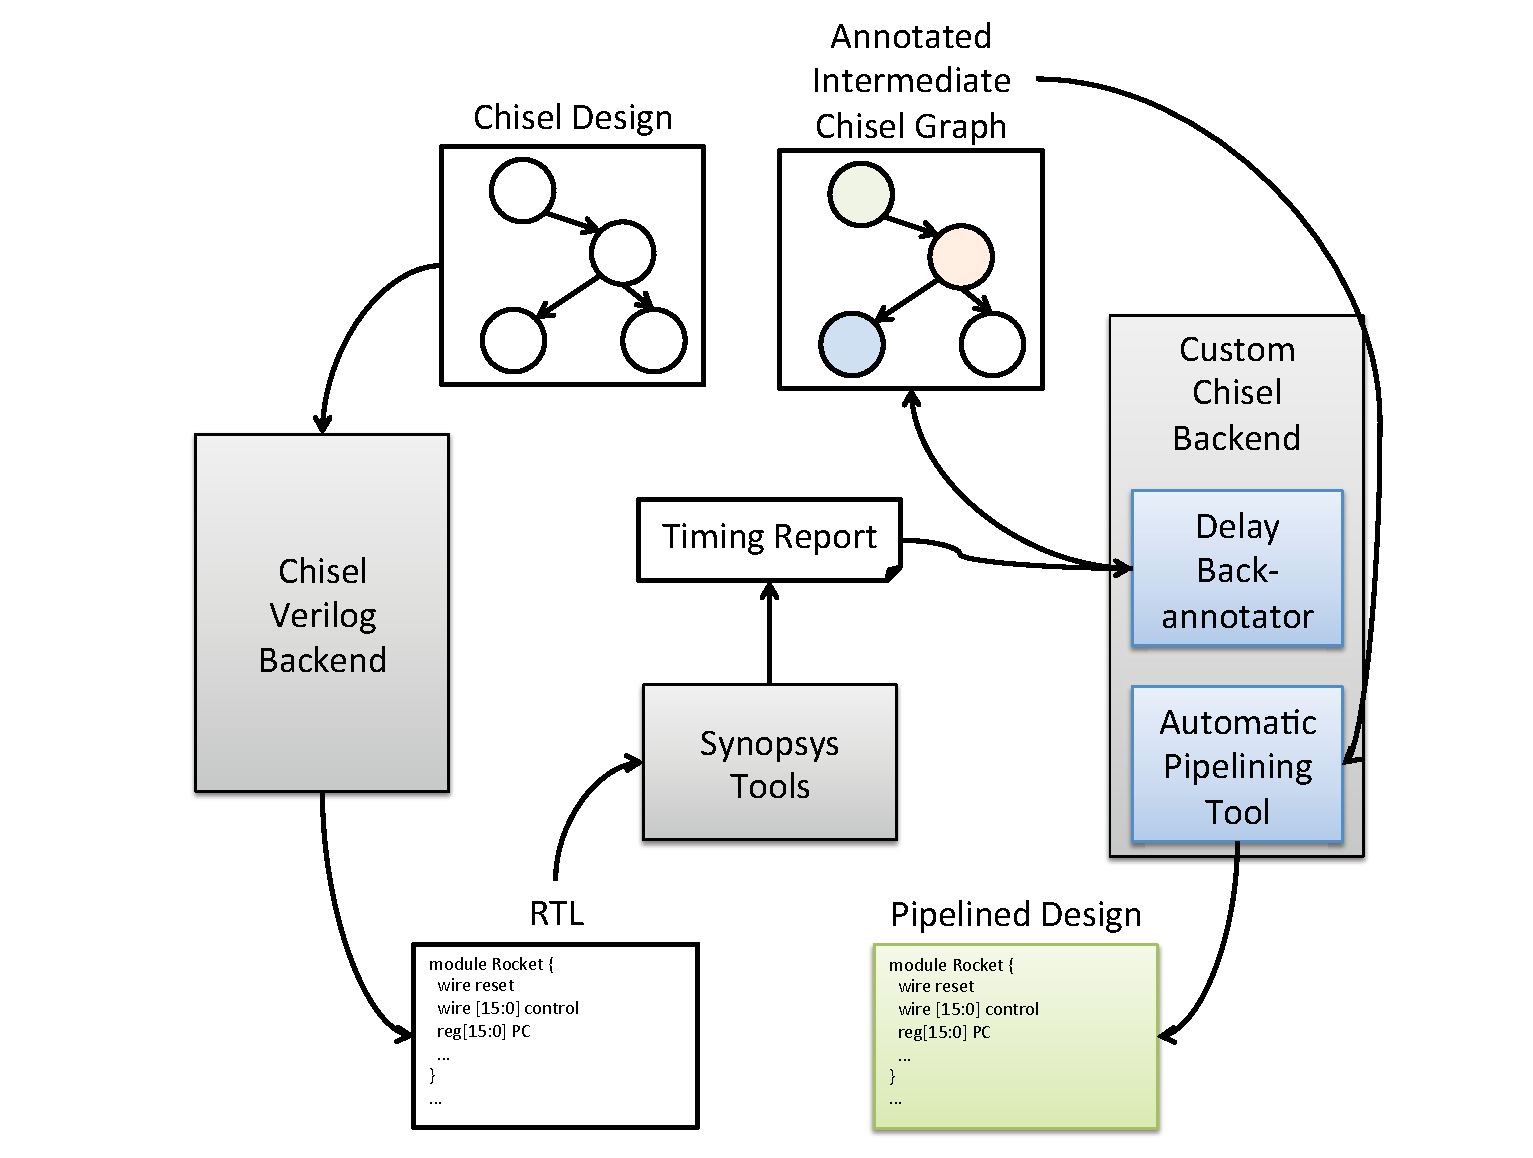
\includegraphics{figures/toolflow}}
    \caption{The overall tool flow}
	\label{fig:toolflow}
\end{figure*}
ßß
\section{Tool Flow}
Figure \ref{fig:toolflow} shows the flow of the entire systems. As the first step, we executes the Chisel Verilog backend which translates a Chisel design into an RTL. The RTL will be used by Synopsys tools to generate timing reports. This is preparation for the second backend execution.

The second backend execution produces an automatically pipelined design from the original Chisel design. We define a customized Chisel backend to include the delay backannotator and the automatic pipelining tool and then execute it after the first run of the Verilog backend. In the second backend execution, the delay backannotator calls Synopsys tools to produce timing reports. It then annotates the intermediate Chisel graph, which is explained in Section \ref{sec:challenges}, by reading the timing reports. The automatic pipelining tool uses the annotated graph to locate the pipeline registers at the optimal places, producing an automatically pipelined design.